\chapter{Analysis}
When working with distance measurement one has to consider different opportunities, and so did we.
Mainly distance can be measured with a method falling into one of two categories:
\begin{itemize}
\item Ruler-method
\item Travel-method
\end{itemize}
\section{Distance measurement}
A simple way to measure distance is to send out some kind of signal, measure the time it is travelling and then calculating the distance using the speed of the signal.
\subsection{Ruler-method}
The ruler-method is measuring a distance relative to a known length and is ancient. The most well-known object used for that is the ruler (hence the name). By comparing a known distance to an unknown one, one can through several different approaches measure the distance.

\subsection{Travel-method}
The travel method is used when the ruler-method is not an option. When using the travel-method, an object must travel the distance one want to measure at a known velocity. By measuring the time it took for the object to travel the distance, the distance can be calculated by dividing the speed by the time it took. This is e.g. used in GPS-applications.

In our application we can quickly rule out the ruler-method as the method would not be convenient to use in an application like ours as it needs to be agile and flexible. Therefore we looked deeper into the travel-method category.
In physics, there are two well-known types of speed: 
\begin{itemize}
\item Speed of light
\item Speed of sound
\end{itemize}
Both are affected by the medium but otherwise constant. Measuring speed of light would require special equipment not immediately at hand. The group had a desire to work with sound and had the equipment at hand. Speed of sound was choosen.

\section{Sound}
Sound is motion of materials/mediums. By motion we mean in frequency. Sound can travel through all mediums and have different speeds depending of this medium. Sound is easy to analyse since we have a lot of tools (fourier transform, spectrum analysing, plot etc) to determine delays or frequency composition.

\subsection{Speed of sound}
To calculate the speed of sound it is important to know the temperature, presure, humidity and gas/medium. The group didn't bother to analyse the complex formulas taking all these factors into account. We found a general formula for the speed of sound in dry air\\
The speed of sound in dry air can be calculated by:
\begin{equation}
c_air=(331.3+0.606*t)\frac{m}{s}
\end{equation}
Where t is the degrees in Celsius. This means the appoximate speed of sound at room temperature is arround $343\frac{m}{s}$.\\
\subsection{Ultrasound}
The ultrasonic sound band is all sound frequencies above 20kHz. Below is ilustrated where the different frequencybands are located and what their names are.
\begin{figure}[H]
\centering
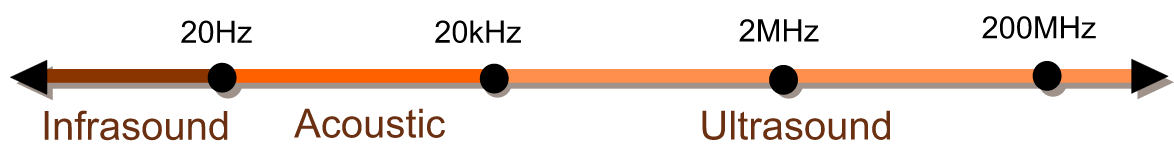
\includegraphics[width=0.6\textwidth]{billeder/frequencybands.png}
\end{figure}
Because ultrasound is at such high frequencies it is quite ideal for an application as ours since it isn't in the hearable range adn therefore wouldn't interfere with the sound from the instrument. Since ultrasound is at >20kHz it also isn't subject to much noise since not many things oscillate at this frequency.\\
The problem about ultrasound is the equipment. It is not possible to simply use ultrasound since we need special speakers and microphones to record and play in these frequencies and this equipment wasn't at hand at the time.
\subsection{Hearable sound}
Sound in the hearable band (20Hz-20kHz) is a bit easier to work with of several reasons. Since it is actually possible to hear what is going on it might be easier to determine problems. We have a lot of equipment ready, speakers and microphones, which is built to these specific frequencies.